\documentclass{article} % Définition de la classe du document (article, report, book, etc.)

% Packages et paramètres supplémentaires
\usepackage[utf8]{inputenc} % Encodage des caractères (UTF-8 recommandé)
\usepackage[T1]{fontenc} % Encodage de la police
\usepackage[french]{babel} % Langue du document (français)
\usepackage{amsmath, amssymb} % Packages mathématiques
\usepackage{graphicx} % Pour inclure des images
\graphicspath{ {./images/} }
\usepackage{cite} % Gestion des citations bibliographiques
\usepackage{hyperref} % Liens hypertextes
\usepackage{nameref}
\usepackage{listings} % Pour inclure du code source
\usepackage{xcolor}

\definecolor{codegreen}{rgb}{0,0.6,0}
\definecolor{codegray}{rgb}{0.5,0.5,0.5}
\definecolor{codepurple}{rgb}{0.58,0,0.82}

\lstdefinestyle{mystyle}{
    commentstyle=\color{codegreen},
    keywordstyle=\color{magenta},
    numberstyle=\tiny\color{codegray},
    stringstyle=\color{codepurple},
    basicstyle=\footnotesize,
    breakatwhitespace=false,
    breaklines=true,
    captionpos=b,
    keepspaces=true,
    numbers=left,
    numbersep=5pt,
    showspaces=false,
    showstringspaces=false,
    showtabs=false,
    tabsize=2
}

\lstset{style=mystyle}

% Titre du document, auteur et date
\title{Architectures Distribué - Java RMI}
\author{GARCIA PENA Loris}
\date{\today} % Utilisez \date{} pour spécifier une date personnalisée

\begin{document} % Début du contenu du document

\maketitle % Génère le titre du document

% Résumé du document
\begin{abstract}
    Ce rapport présente notre travail réalisé dans le cadre du TP1 portant sur Java RMI (Remote Method Invocation). Le TP1 avait pour principaux objectifs :

    \begin{itemize}
        \item Comprendre la notion d'objet distribué.
        \item Utiliser le passage de stub ou d'objet sérialisé.
        \item Explorer le téléchargement de code via l'utilisation de la codebase.
    \end{itemize}
\end{abstract}

% Table des matières (générée automatiquement)
\tableofcontents

\newpage % Nouvelle page pour la première section

\section{Introduction}

La technologie Java Remote Method Invocation (RMI) est un système puissant qui permet à un objet s'exécutant dans une machine virtuelle
Java d'invoquer des méthodes sur un objet s'exécutant dans une autre machine virtuelle Java distante. Cette capacité de communication à distance
entre des programmes repose sur l'invocation de méthodes sur des objets distribués appellés stub.
En d'autres termes, elle offre la possibilité d'interagir avec un objet distant comme s'il était local.
Cela favorise la construction d'applications réparties en utilisant des appels de méthode au lieu d'appels de procédure,
simplifiant ainsi le développement d'applications distribuées.

Dans le cadre de ce projet, nous nous plaçons dans le contexte d'un cabinet vétérinaire.
Chaque patient du cabinet, c'est-à-dire chaque animal, possède une fiche individuelle avec un dossier de suivi médical.
L'objectif est de créer un système où chaque vétérinaire du cabinet peut accéder aux fiches des patients à distance.
Nous mettrons en place un serveur et développerons un client pour les vétérinaires.

\newpage
\section{Architecture globale}

L'architecture globale de notre système repose sur trois composants principaux :
\begin{itemize}
    \item Une partie Serveur, responsable de la gestion du cabinet medical.
    \item Une partie Client, utilisée par les vétérinaires pour accéder au cabinet medical.
    \item Une partie commune (\textit{Common}), qui permet de structurer les composants communs.
\end{itemize}

\begin{figure}[h]
    \centering
    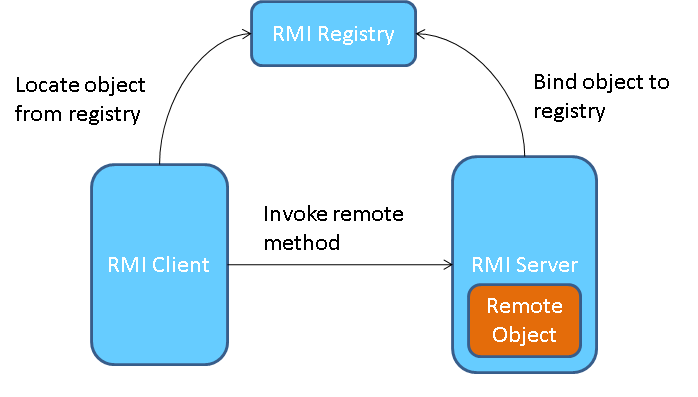
\includegraphics[width=0.8\textwidth]{rmi}
    \caption{JAVA RMI}
    \label{fig:schema-rmi}
\end{figure}

Cette architecture permet la création d'une application distribuée utilisant Java RMI 
pour la communication à distance. Chaque composant joue un rôle essentiel dans le fonctionnement 
de notre application vétérinaire.
Dans notre application, chaque composant est implémenté en tant que projet distinct.

\subsection{Partie Serveur}

Le serveur est responsable de la création d'objets, dans notre cas, le cabinet médical, 
qui sont rendus disponibles pour l'accès distant via Java RMI. 
Le serveur crée ces objets et les publie dans un registre RMI. 
Le registre RMI agit comme un annuaire central permettant aux clients d'accéder aux objets distants.

Ainsi, le serveur joue un rôle essentiel dans la mise en place de l'infrastructure RMI, 
permettant aux différentes clients (vétérinaire) d'accéder aux différentes fonctions disponibles 
dans le cabinet médical. Il met en place une communication sécurisée entre les clients 
et les objets distants (stub). 
Le serveur gère également la gestion des \nameref{sec:callback} pour alerter les clients lorsque 
certains seuils sont atteints, améliorant ainsi la réactivité et la gestion du cabinet médical.

\subsection{Partie Clients}

Le composant client de notre projet est destiné aux vétérinaires du cabinet. 
Chaque vétérinaire utilise un client pour interagir avec le cabinet vétérinaire à distance.
Lorsqu'un vétérinaire effectue une opération, le client communique avec le serveur en utilisant Java RMI.

Chaque client utilise un objet stub pour représenter l'interface distante de notre cabinet médical. 

L'objet stub agit comme un proxy local pour l'objet distant du serveur. 
Lorsqu'un client appelle une méthode sur l'objet stub, la requête est automatiquement acheminée vers le serveur.

Les clients utilise une interface en ligne de commande (CLI) pour effectuer diverses actions, 
telles que la recherche de patients, l'ajout de nouveaux animaux, la consultation des dossiers médicaux, 
etc.

De plus, les clients utilisent des méthodes qui déclenchent des affichages dans le terminal du serveur, 
permettant aux vétérinaires de rester informés en temps réel sur les opérations effectuées sur le cabinet médical.

Enfin, les clients déposent les fichiers de classes (`.class`) dans un répertoire `codebase`, 
permettant ainsi au serveur de les télécharger et de les rendre accessibles (voir section \nameref{sec:codebase}).

\subsection{Partie commune (\textit{Common})}

Le module commun, également appelé \textit{Common}, est utilisé en tant que 
composant partagé entre le serveur et les clients. 
Il contient les classes et interfaces nécessaires à la communication entre le serveur et les clients. 
En utilisant ce module, nous garantissons la cohérence des données partagées et 
simplifions le développement en évitant la duplication de code. 

Le module commun contient des définitions d'objets partagés, telles que les interfaces des différents 
objets distribués, mais aussi des classes partagées. 

\bigskip
\textbf{Conclusion}
\bigskip

L'architecture de notre projet basé sur Java RMI offre donc une solution robuste 
pour la gestion d'un cabinet vétérinaire à distance. 
Elle se compose de trois parties, chacune de ces parties remplit un rôle distinct, 
contribuant ainsi à la création d'une application distribuée fonctionnelle.

Le serveur centralise la création et la gestion des objets distants, 
tandis que les clients utilisent des objets stub pour interagir avec l'interface distante. 
L'architecture garantit une communication à distance fluide et sécurisée.

En résumé, l'architecture globale de notre projet simplifie la gestion des 
opérations vétérinaires à distance.

\newpage
\section{Communication}

La communication dans notre application Java RMI repose sur le mécanisme de 
communication à distance offert par RMI. 
Elle permet aux vétérinaires (clients) d'interagir avec le cabinet médical (serveur) 
de manière transparente, comme s'ils travaillaient en local.

\subsection{Invocation de Méthodes à Distance}

L'invocation de méthodes à distance est la base de la communication dans notre application. 
Grâce à Java RMI, les vétérinaires peuvent invoquer des méthodes 
définies dans l'interface \texttt{ICabinetMedical} sur des objets distants situés côté serveur. 
Ces méthodes permettent d'ajouter, chercher, supprimer des animaux, etc.

Lorsqu'un vétérinaire appelle l'une de ces méthodes, 
RMI utilise automatiquement un objet stub pour gérer la communication à distance. 
Les paramètres sont sérialisés, les appels sont acheminés vers le serveur, 
et les résultats sont renvoyés au client. Cette approche rend la communication à distance transparente 
et simplifie la gestion des opérations à travers des objets proxy locaux.

\subsection{Sérialisation des objets dans l'application RMI}

L'un des aspects clés de notre application Java RMI réside dans la 
capacité à transmettre des objets d'une machine virtuelle Java à une autre de 
manière transparente. Cela est rendu possible grâce au mécanisme de sérialisation de Java.

\subsection{Mécanisme de sérialisation de Java}

La sérialisation est un processus par lequel un objet Java est converti en un flux d'octets, 
ce qui permet de le transférer sur un réseau ou de le stocker dans un fichier. 
La désérialisation est le processus inverse, où un flux d'octets est converti en un objet Java. 
Java fournit un mécanisme de sérialisation intégré qui facilite grandement la communication entre 
les machines virtuelles.

\begin{figure}[h]
    \centering
    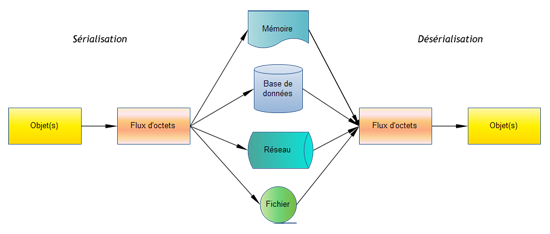
\includegraphics[width=1\textwidth]{serialisation}
    \caption{Sérialisation dans une application}
    \label{fig:serialisation}
\end{figure}

Dans notre applicatio, lorsque nous passons des objets tels que des patients 
ou des espèces entre le serveur et les clients, 
Java gère automatiquement la sérialisation et la désérialisation. Cela simplifie considérablement 
le processus de développement, car les détails de la sérialisation ne nécessitent pas 
d'intervention directe de notre part.

En résumé, la sérialisation est un composant essentiel de notre application RMI, 
qui permet la transmission des objets entre le serveur et les clients. 
Grâce à l'héritage de la classe \texttt{UnicastRemoteObject}, 
les objets de la classe \texttt{CabinetMedical} peuvent être sérialisés et désérialisés, 
contribuant ainsi à la robustesse de notre système distribué.

\subsection{Sérialisation implicite}

Dans notre application, la classe \texttt{CabinetMedical} est un composant central qui gère 
les dossiers des patients. Bien que cette classe n'implémente pas directement l'interface \texttt{Serializable}, 
elle bénéficie de la sérialisation grâce à l'extension de la classe \texttt{UnicastRemoteObject}. 
Cette extension rend les objets de la classe \texttt{CabinetMedical} sérialisables, 
ce qui est essentiel pour la communication distante via RMI. 
Ainsi, lorsqu'un objet \texttt{CabinetMedical} est transmis entre le serveur et les clients, 
il est automatiquement sérialisé et désérialisé.
Nous avons également implémenté une classe \texttt{Espece} qui étend directement \texttt{Serializable}. 
Permettant au serveur de sérialiser et de désérialiser les objets de cette classe. 

\newpage
\section{Sécurité et codebase}\label{sec:codebase}

La sécurité est un aspect crucial de toute application distribuée, 
et Java RMI offre des mécanismes intégrés pour la gestion de la sécurité. 
Dans notre projet, nous avons commencé à mettre en place des mesures de sécurité de base.

\subsection{Politique de Sécurité}

\begin{sloppypar}
    Nous avons configuré une politique de sécurité en utilisant le fichier \texttt{security.policy}. 
    Cette politique définit les autorisations et les restrictions qui seront appliquées aux 
    composants de notre application. La politique de sécurité est chargée via la ligne de code suivante :
\end{sloppypar}

\begin{lstlisting}[language=Java]
System.setProperty("java.security.policy", "security/security.policy");
\end{lstlisting}


Dans le fichier de politique de sécurité, situé coté serveur dans un sous dossier security, 
nous avons actuellement octroyé toutes les autorisations 
à notre application en utilisant la règle suivante :

\begin{lstlisting}
grant {
    permission java.security.AllPermission;
};
\end{lstlisting}

Cela signifie que notre application a la permission d'accéder à toutes les ressources 
et d'effectuer toutes les actions, ce qui est une configuration très permissive et ne 
devrait être utilisée que pour des besoins de développement et de test.

Dans un environnement de production, il est fortement recommandé de définir des politiques de sécurité 
plus restrictives pour protéger les ressources sensibles et garantir l'intégrité de l'application.

\subsection{Gestionnaire de Sécurité}

Nous avons également mis en place un gestionnaire de sécurité avec la ligne de code suivante :

\begin{lstlisting}[language=Java]
System.setSecurityManager(new SecurityManager());
\end{lstlisting}

Le gestionnaire de sécurité est responsable de l'application des politiques de sécurité définies. 
Il veille à ce que les actions de l'application soient conformes aux autorisations spécifiées 
dans la politique de sécurité.

Bien que notre configuration actuelle soit permissive pour faciliter le développement, 
il est essentiel de noter que dans un environnement de production, des politiques de sécurité 
appropriées doivent être définies pour protéger l'application contre les menaces potentielles.

\newpage
\section{Diagrammes de Conception}

Le diagramme de classes présenté ci-dessous (Figure \ref{fig:diagramme-classe}), 
offre une vue globale des relations entre les composants clés de notre projet, 
notamment les classes, les interfaces, et les flux de données. 

\begin{figure}[h]
    \centering
    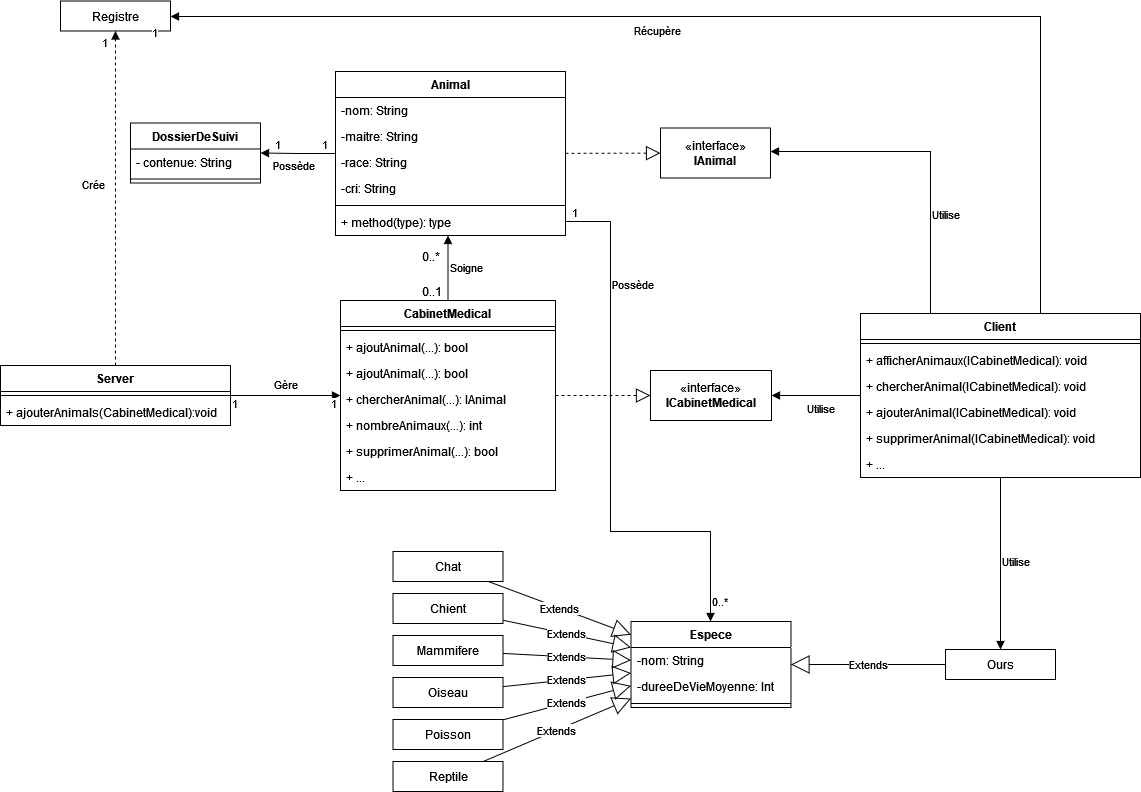
\includegraphics[width=1\textwidth]{classe}
    \caption{Diagramme de classes}
    \label{fig:diagramme-classe}
\end{figure}

Le diagramme de classes met en évidence un élément essentiel de notre architecture Java RMI : 
le registre RMI. Le registre RMI joue un rôle crucial en servant de répertoire 
central pour la publication des objets distants. 
Cela permet aux clients d'accéder facilement aux objets distants 
en utilisant un mécanisme de recherche. 
La présence du registre RMI dans notre diagramme souligne son rôle 
fondamental dans la mise en place de la communication à distance au sein de notre application, 
renforçant ainsi la gestion des objets distants et des clients.


\newpage
\section{Composants clés}

Pour comprendre en détail les composants clés de notre application Java RMI, examinons les principales classes et interfaces qui les composent.

\subsection{Composants communs (Côté Common)}


\textbf{· Interface IAnimal}
\bigskip

L'interface \texttt{IAnimal} est une interface distante qui définit les méthodes que tout animal doit mettre en œuvre. Elle étend l'interface \texttt{Remote}, ce qui permet aux objets qui la mettent en œuvre d'être distribués via Java RMI. Cette interface définit des méthodes pour obtenir le nom de l'animal, afficher des informations sur l'animal, émettre un cri, consulter le dossier de suivi, obtenir des informations sur l'espèce de l'animal, etc.

\textbf{· Interface ICabinetMedical}
\bigskip

\textbf{· Classe Espece}
\bigskip

La classe \texttt{Espece} est un composant commun qui définit une espèce d'animal. Elle implémente l'interface \texttt{Serializable} pour permettre la sérialisation des objets lors de la communication à distance. Cette classe contient des propriétés telles que le nom de l'espèce et la durée de vie moyenne. Elle joue un rôle crucial pour définir les caractéristiques des animaux au sein du système.

L'interface \texttt{ICabinetMedical} est le pilier central de notre système. Elle définit les services que le cabinet médical offre aux vétérinaires. Cette interface distante expose des méthodes pour ajouter des animaux, chercher des animaux, supprimer des animaux, obtenir la liste des patients, et bien plus encore. Elle permet également d'enregistrer des callbacks pour les alertes.

\subsection{Composants serveur}

\textbf{Classe Animal}
\bigskip


La classe \texttt{Animal} est une implémentation de l'interface \texttt{IAnimal}. Elle représente un patient du cabinet vétérinaire et stocke des informations telles que le nom, le maître, l'espèce, la race, le cri et le dossier de suivi de l'animal. Cette classe est utilisée côté serveur pour créer et gérer les fiches médicales des animaux.

\textbf{Classe CabinetMedical}
\bigskip


La classe \texttt{CabinetMedical} est le cœur du côté serveur. Elle gère une liste d'animaux (patients) au sein du cabinet médical. Cette classe expose les méthodes définies dans l'interface \texttt{ICabinetMedical} pour gérer les patients, rechercher des animaux, supprimer des patients, et plus encore.

\subsection{Composants client}

\textbf{Classes Ours et Client}
\bigskip

Côté client, nous trouvons la classe \texttt{Ours} qui hérite de la classe \texttt{Espece}. Elle représente une espèce spécifique (l'ours) et est utilisée pour créer des animaux de cette espèce.

La classe \texttt{Client} est responsable de l'interaction des vétérinaires avec le cabinet médical. Elle propose plusieurs fonctions, notamment l'affichage des animaux, la recherche, l'ajout et la suppression d'animaux. Les vétérinaires utilisent cette classe pour gérer les fiches médicales des patients du cabinet vétérinaire.

\subsection{Résumé}

Les composants clés de notre application Java RMI comprennent des classes telles que \texttt{Espece}, \texttt{Animal}, \texttt{CabinetMedical}, des interfaces comme \texttt{IAnimal} et \texttt{ICabinetMedical}, ainsi que des classes spécifiques aux espèces d'animaux comme \texttt{Ours}. Ces éléments interagissent pour permettre la gestion des fiches médicales des patients et la communication à distance entre les vétérinaires et le cabinet médical. Ils jouent un rôle essentiel dans la réalisation des objectifs de notre projet Java RMI.

\section{RMI Callback}\label{sec:callback}

Dans notre application Java RMI, nous utilisons le mécanisme de callback pour informer les clients des seuils atteints en matière de nombre de patients dans le cabinet médical. Cette fonctionnalité est essentielle pour alerter les vétérinaires lorsqu'un certain nombre de patients est atteint.

\bigskip
\textbf{Côté client :}

Dans le package \texttt{com.cabinet.common.rmi}, nous avons défini l'interface \texttt{IClientCallback}, qui étend l'interface \texttt{Remote}. Cette interface contient une méthode, \texttt{notifierSeuilAtteint}, qui est appelée par le serveur pour notifier un client de l'atteinte d'un seuil.

\bigskip
\textbf{Côté serveur (dans CabinetMedical) :}

Nous avons une liste, \texttt{listeClients}, qui stocke les clients enregistrés pour les notifications de seuil. Le serveur offre une méthode, \texttt{enregistrerAlertCallback}, qui permet d'enregistrer un client pour les alertes. Si un client n'est pas déjà enregistré, il est ajouté à la liste.

\bigskip
\textbf{Côté client :}

Dans le package \texttt{com.cabinet.client.rmi}, nous avons implémenté la classe \texttt{ClientCallbackImpl} qui étend \texttt{UnicastRemoteObject} et implémente l'interface \texttt{IClientCallback}. Cette classe fournit l'implémentation de la méthode \texttt{notifierSeuilAtteint}, qui affiche une alerte sur la console client indiquant le nombre de patients atteint.

Dans \texttt{Client.java}, nous créons une instance de \texttt{ClientCallbackImpl} et l'enregistrons auprès du serveur en appelant la méthode \texttt{enregistrerAlertCallback} du cabinet médical.


Ce mécanisme de callback permet aux clients d'être informés en temps réel des seuils atteints et d'agir en conséquence.


\end{document} % Fin du document
